\documentclass[../../main.tex]{subfiles}

%-----------------------------------------------------------%
\begin{document}
\subsection{Tracking Mode}

\subsubsection{Introduction}
Tracking Mode is the primary operating mode of a satellite (the other being the Lost-in-Space Mode, which is generally a rare event in the lifetime of a standard operating star tracker), wherein the attitude of the satellite is already known. The main objective of tracking mode is to perform Star Matching using the \textit{a priori} attitude information to decrease the computation time as compared to the Lost-in-Space Mode for successfully matching observed stars with their true Star-IDs (from the pre-loaded Star Catalogue). 

\subsubsection{Literature Survey}
After an extensive literature survey on Tracking Mode algorithms, a few algorithms were shortlisted based on the number of citations, space heritage, ease of implementation and the year of publication. Some papers were survey based papers which documented an extensive study on different algorithms proposed till date. Many algorithms were shortlisted based on the results shown in these papers. These algorithms are mentioned in detail below. 

\subsubsection{Recursive Mode Star Identification Algorithms}
% hey, don't write "This Paper", instead write "This algorithm \cite{ref} proposes ...."
This paper proposes two methods for recursive mode star identification, the Spherical Polygon search (SP-search) and the Star Neighbourhood Approach (SNA). Once the Lost-in-Space Algorithm (LISA) has been executed for a single frame of the star tracker, the proposed algorithm (SNA or SP Search) is used to obtain expected stars in the FOV from the Star Catalogue for the next frame. These expected stars form the \textit{Reference Image}.
The Feature Extraction process is executed in the next frame, obtaining the true centroids, which form the \textit{Measured Image}.The Star ID process is completed by matching the inter-star angles between the measured image and the reference image. The two algorithms are explained in detail below. 
\begin{itemize}
    \item \textbf{Spherical Polygon Approach}\\
    \\
    The Spherical Polygon Approach does not require any (accurate or not) initial guess of the spacecraft attitude, and does not use the typically low accuracy magnitude information. The algorithm is recursive in the sense that it matches 3 stars at a time observed in the \textit{Measured Image} till all the observed stars are matched. 
   If \textit{$s_{i}$}, \textit{$s_{j}$}, and \textit{$s_{k}$} are three different observed star directions (unit-vectors), it is always possible to set
   \begin{equation}
        \textit{$s_{k}$} = a\textit{$s_{i}$} + b\textit{$s_{j}$} +c(\textit{$s_{i}$} \times \textit{$s_{j}$})
    \end{equation}
    unless \textit{$s_{i}$} and \textit{$s_{j}$} are not parallel (i.e. double stars). The a, b and c coefficients represent an invariant set of parameters with respect to the used system of coordinates. This means that there exists, in the Star Catalogue, three stars (\textit{$v_{i}$}, \textit{$v_{j}$} and \textit{$v_{k}$}) such that condition (10.1) holds as,  
    \begin{equation}                    
        \textit{$v_{k}$} = a'\textit{$v_{i}$} + b'\textit{$v_{j}$} +c'(\textit{$v_{i}$} \times \textit{$v_{j}$})
    \end{equation}
    where the a', b', and c' coefficients will differ from the a, b, and c coefficients because of the sensor’s limited precision, that is, because the observed stars directions do not perfectly overlap with the catalog star directions.\\
    The algorithm uses the \textbf{K-vector} (Refer \ref{appendix:k-vector}) range searching technique twice to finally match a triad of observed stars. Based on these facts, the algorithm follows the following steps:
    \begin{enumerate}                   
        \item The first instance of the use of \textbf{K-vector} is to find all the catalogue star pairs (\textit{$v_{i}$} and \textit{$v_{j}$}) admissible with the observed star pair \textit{$s_{i}$} and \textit{$s_{j}$}.
        \item For each possible pair of catalogue stars, there exists a corresponding solution for the true catalogue star \textit{$v_{k}$} associated with the observed \textit{$s_{k}$} star.
        \item To find the true solution for \textit{$v_{k}$} out of all possible solutions, it has to be searched within a cone of aperture h$\sigma$ around each solution, which is done using the \textbf{\textit{k}-vector} technique.
        \item This is accomplished by approximating the observed cone area as the area covered by a spherical polygon, which is identified as the intersection of six cones, as shown in fig. 10.6
        \item The SPS procedure has a successful end if only one star falls within one of the cones of aperture h$\sigma$. When this occurs, the triad (\textit{$s_{i}$}, \textit{$s_{j}$}, \textit{$s_{k}$}) is matched with the triad (\textit{$v_{i}$}, \textit{$v_{j}$}, \textit{$v_{k}$}). 
    \end{enumerate}
    \begin{figure}[!h]
        \centering
        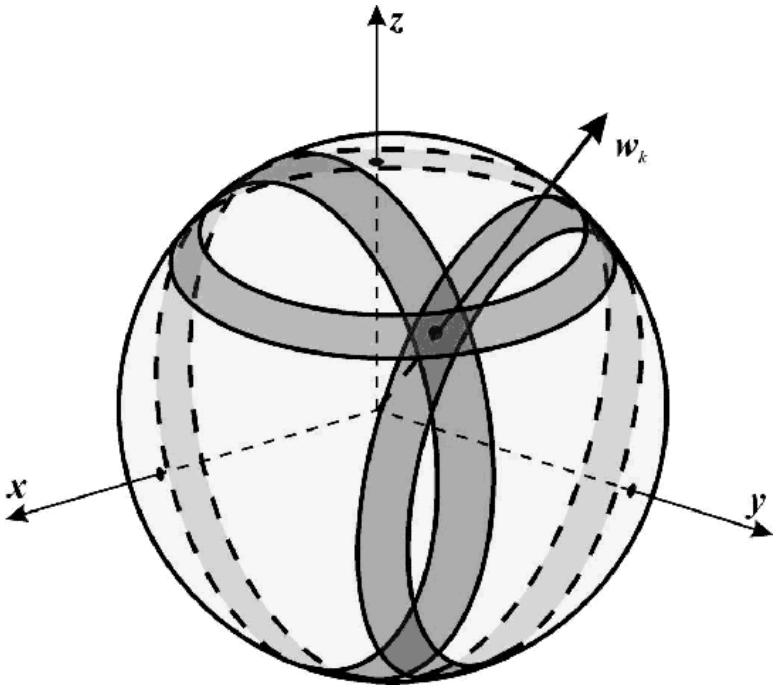
\includegraphics[scale=0.35]{Figures/GNC/sp_search.png}
        \caption{Spherical Polygon}
        \label{fig:sp_search}
    \end{figure}
    
    \item \textbf{Star Neighbourhood Approach} \label{sna}\\
    
    The Star Neighbourhood approach is the second recursive algorithm which uses the previously identified stars to access the candidate stars (which form the \textit{Reference Image}) to match with the current observed stars (which form the \textit{Measured Image}). This approach makes use of the spacecraft attitude at each frame (obtained by estimating the Angular Velocity from the Gyroscope) and the previously identified Star IDs. The steps of the algorithm are detailed below:
    \begin{enumerate}
        \item The LISA is run for the first time which determines the \textbf{attitude matrix} and \textbf{Star-IDs} at time $t_{0}$.
        \item \textbf{Simulation of Stars}
        By knowing the attitude matrix at each time step we can calculate the normal vectors to the sensor frame in the body frame, which is known as the 'Bore-sight vector', to simulate the frames of stars at the next time step, i.e, create a simulation of the actual image which will contain catalogue stars and place them at positions at which the 'true centroids' should ideally be found (\textit{Reference Image}).
        \item \textbf{Star Mapping}
        The simulated star unit vectors are converted to image plane coordinates ($x_{i}$, $y_{i}$)using the following formula:
        \begin{equation}
            x_{i} = -f\frac{x^{T}b_{i}}{z^{T}b_{i}} \hspace{3em} y_{i} = -f\frac{y^{T}b_{i}}{z^{T}b_{i}}
        \end{equation}
        where \textbf{$C^{T}$ = [x,y,z]} is the sensor attitude matrix, \textbf{$b_{i}$ (i=1,2,3.....n)} are the simulated star vectors and \textbf{f} is the camera focal length. 
        \item \textbf{Star Spot Prediction}
        The estimated location of star i at the current frame ($x_{i}$, $y_{i}$)$_{t+\delta t}$ is calculated by adding the location of star i at the previous frame ($x_{i}$, $y_{i}$)$_{t}$ and estimated translation of the frame $\omega\delta$t.
        \item \textbf{Star Matching} Now the estimated locations of stars (Reference Image) is matched with the measured locations of stars (Measured Image) using a Radius based approach with \emph{Matching Radius} equal to $3\sqrt{2}\sigma$ as shown in figure (10.7). 
        \begin{figure}[!h]
        \centering
        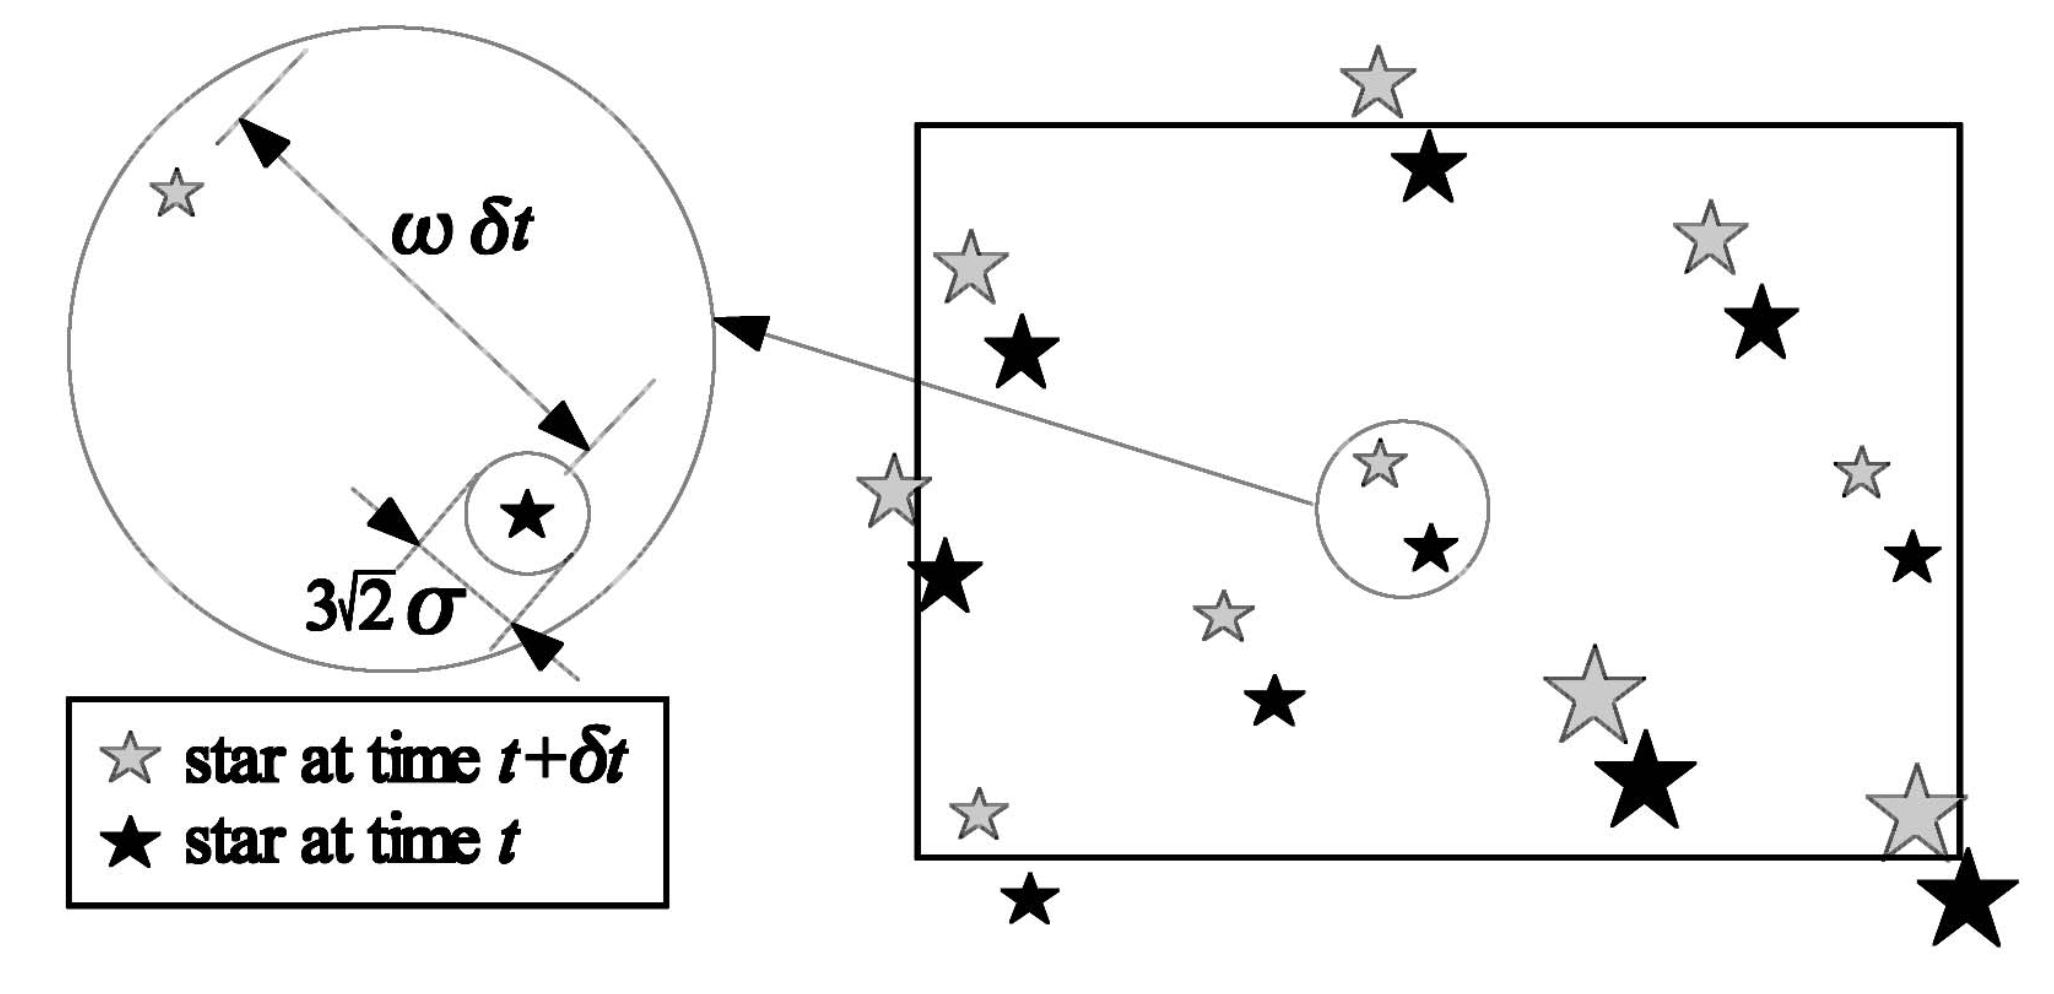
\includegraphics[scale=0.20]{Figures/GNC/radius_matching.png}
        \caption{Radius Based Matching}
        \label{fig:radius_based_sna}
        \end{figure}
        \item For the unmatched stars from steps 4 and 5, the \textbf{Star Neighbourhood Table} is used to identify the stars which enter the sensor frame at ($t+\delta t$), by checking the inter-star angles between the unmatched stars and their matched star neighbours. 
    \end{enumerate}
    The logic for the SNA is as follows (\ref{fig:sna_flowchart}):
    
    \begin{Flowchart}
        \centering
        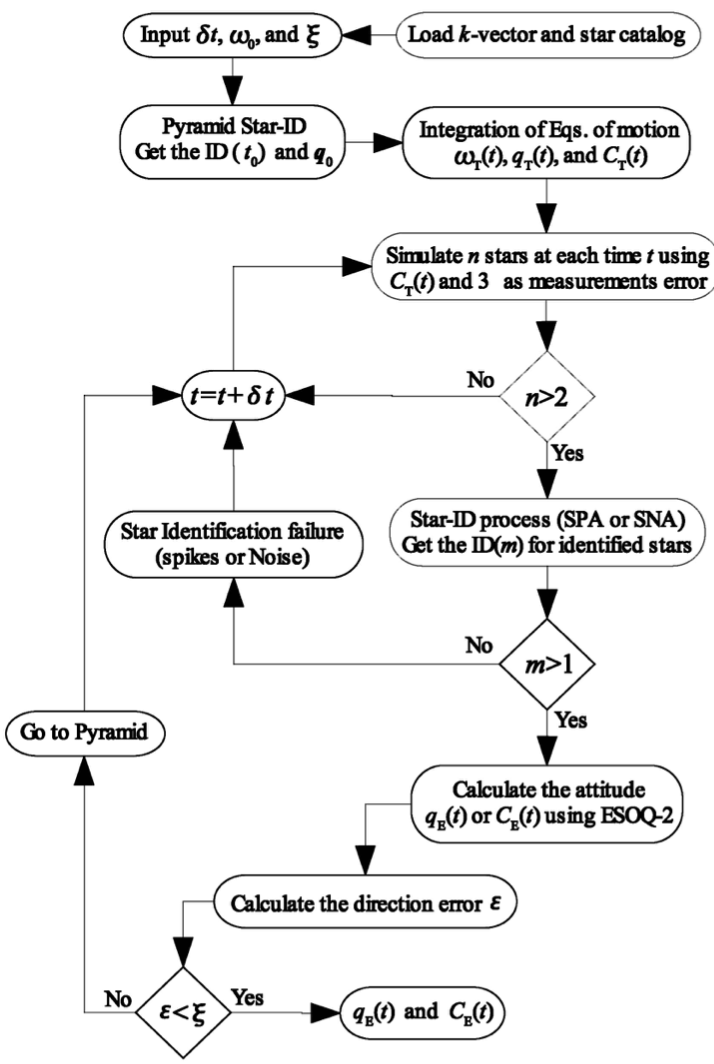
\includegraphics[scale=0.55]{Figures/GNC/sna_flowchart.png}
        \caption{SNA algorithm}
        \label{fig:sna_flowchart}
    \end{Flowchart}
\end{itemize}

\subsubsection{Rapid Star Tracking Algorithm} \label{rapidtrack}
This algorithm does not require any previous attitude information or an estimate of the angular velocity of the spacecraft, unlike the previous algorithm. Instead, it only uses the previously identified stars' information (Right Ascension, Declination, Star ID) to track stars in the current frame. Before understanding the details of the algorithm, some terms are introduced:
\begin{itemize}
    \item \textbf{Reference Image} : The image from the previous frame where all the observed stars have been identified.
    \item \textbf{Observed/Measured Image} : The image at the current frame where only the centroid information is known, and the task at hand is to correctly identify these centroids using the information of the Reference Stars (in the Reference Image). 
\end{itemize}
The principle of the algorithm is detailed step-by-step below:
\begin{enumerate} \label{rapid_explain}
    \item The star images at the $(k-1)^{th}$ frames and before have been identified, and the objective is to identify the Observed Image at $(k)^{th}$ frame. The identified star image at $(k-1)^{th}$ frame is considered as the Reference Image for the $(k)^{th}$ frame. 
    \item The euclidean distance between the stars in the two images is calculated and compared with a \textbf{radius r}, known as the matching radius, to determine if any reference stars fall in the neighbourhood of an observed star, and if yes, how many. 
    \item If a star's neighborhood in the observed image includes only one star in reference image, the star in observation image is matched with the star in reference image and the star in the observation star image is 'tracked' successfully.
    \item If a star's neighborhood in observation star image includes no
    star or more than one star in reference star image, the star is not matched and tracked. 
    \begin{figure}[!h]
        \centering
        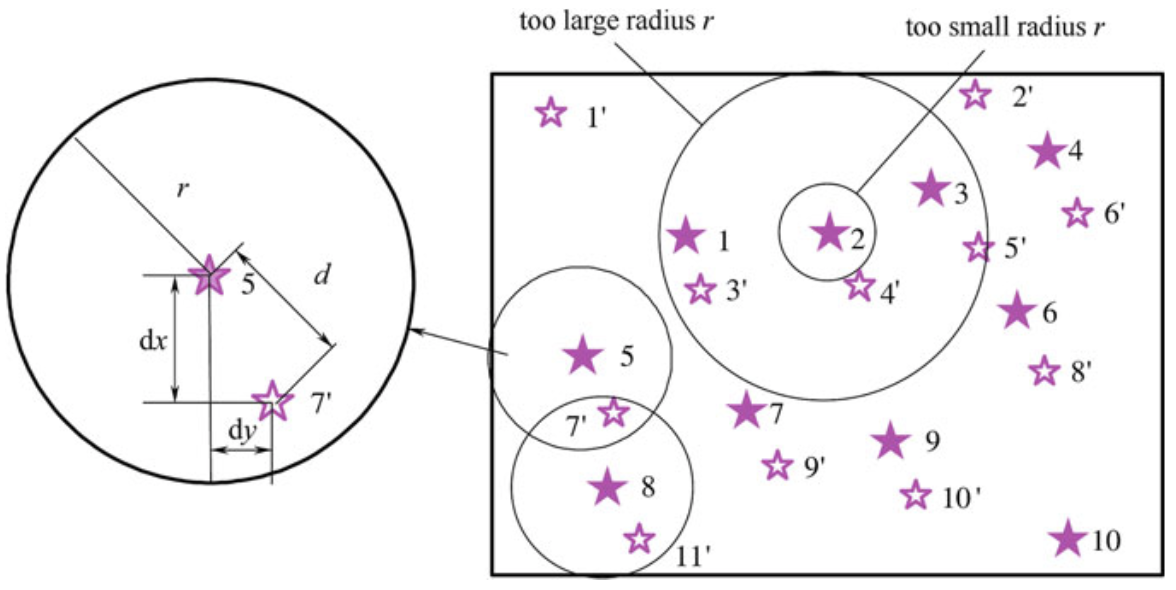
\includegraphics[scale=0.3]{Figures/GNC/radius_based_zhang.png}
        \caption{Radius Based Star Matching}
        \label{fig:radius_zhang}
    \end{figure}
    \item The $(k+1)^{th}$ reference star image can be generated from the tracking results and used to match with the next observation star image in the same way; then stars can be tracked continuously.
    \item Now the stars in the Reference Image will be moved away from the FOV one-by-one. When the stars left in the reference image is less than \textbf{3}, new star identification is necessary, which is done by calculating the star sensor's \textbf{boresight} vector according to the result of the previous tracking, and the stars around the boresight can be obtained from the Star Catalogue.  
    \item The stars vectors obtained from the catalogue in the previous step are obtained from the \textit{Celestial Coordinates} (RA, Dec.) and need to be converted to \textit{Image Plane Coordinates} to start again from step 1. This process is known as \textbf{Star Mapping} is generally a time-consuming task, hence it is executed only when the reference stars are less than 3. 
\end{enumerate}

\begin{Flowchart}
        \centering
        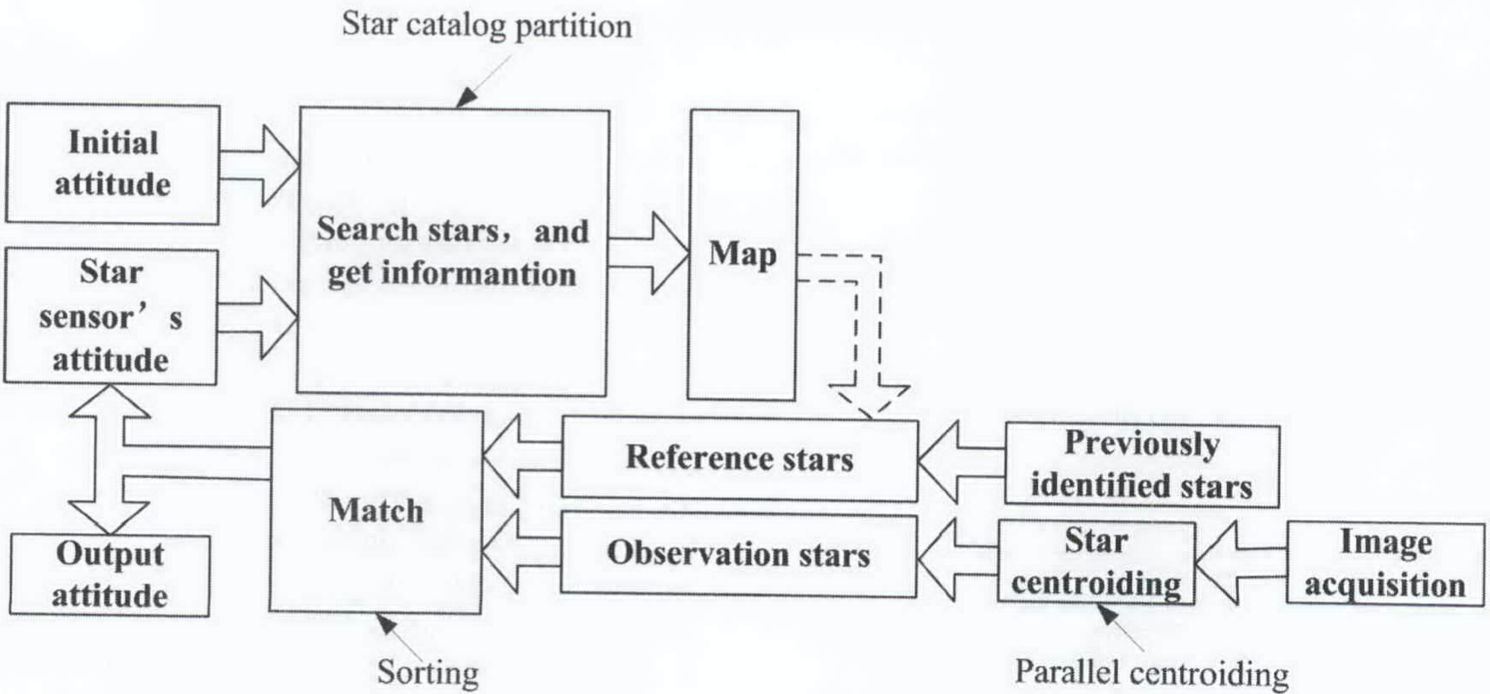
\includegraphics[scale=0.4]{Figures/GNC/rapid_tracking_flowchart.png}
        \caption{Rapid Star Tracking Algorithm}
        \label{fig:rapid_tracking_flowchart}
\end{Flowchart}

To speed up the process of star tracking, the algorithm also proposes 3 optimisation techniques. These are explained below:
\begin{itemize}
    \item \textit{Parallel Star Centroiding}:\\
    This employs the Pixel-by-Pixel centroiding algorithm (Refer \ref{sec:pixel_by_pixel})
    
    \item \textit{Sorting Before Matching} \label{sorting_before_matching}:\\
    % Use the right \ref{} command here
    In step 2 of the algorithm \ref{rapid_explain}, the matching between the stars in observation star image and reference star image is implemented one-by-one. But matching between stars with a long distance is meaningless, so sorting before matching is introduced. That is, the stars in the observation image are sorted in ascending order according to their image plane coordinates using bubble sort, and then the matching is carried out. This decreases the number of operations significantly. 
    
    \item \textit{Star Catalogue Partition} \label{catalogue_partition}:\\
    In step 6 and 7 of the algorithm \ref{rapid_explain}, new star identification is done by accessing catalogue stars using the boresight vector and then mapping them onto the star sensor plane (Star Mapping), which can be time consuming and inefficient if searching for stars through the entire guide star catalogue. This is solved using the concept of \textit{`sub-catalogue'}.
    \begin{itemize}
        \item The celestial sphere is divided into 6 equal zones by using an inscribed cube and then pushing the sides of the cube away from the center of the sphere, to generate 6 equal parts of the celestial spheres. 
        \item Each one of the 6 zones can be partitioned into N x N sub portions. This way, the entire celestial sphere is divided into 6 x N x N sub portions. 
        \item Now all the guide stars can be assigned into these sub portions, instead of their irregular distribution on the whole celestial sphere. This way, if the boresight direction is known in step 6, the sub portion and hence the guide stars around that boresight can be found quickly. The partition table will be pre-processed and stored with the guide catalogue. 
    \end{itemize}
\end{itemize}


\subsubsection{Rapid Star Tracking Using Star Spot Matching Between Adjacent Frames} \label{zhang}
This algorithm is very similar to the `Rapid Star Tracking Algorithm' with a minor difference being in how the \textbf{Reference Image} is formed at every frame. The algorithm introduces another step, known as \textbf{Star Spot Prediction}, which uses the movement of stars in the previous frames to predict the position of stars in the next frame of star image. The flowchart of the algorithm is shown in Fig. \ref{fig:zhang_tracking_flowchart}.\\
In accordance with the attitude of star sensor, boresight vector of the current frame can be calculated, after which the Star ID process is carried out as described in steps 2, 3 and 4 of section \ref{sna}. 
Star matching between the predicted centroids (Reference Image) and the true centroids (Measured Image) is carried out as shown in Fig. \ref{fig:radius_zhang}. A thing to be noted here is that the `Matching Radius' used for star matching in this algorithm will be smaller because the reference stars here are the predicted centroids instead of the identified stars of the previous frame. 
\begin{Flowchart}
        \centering
        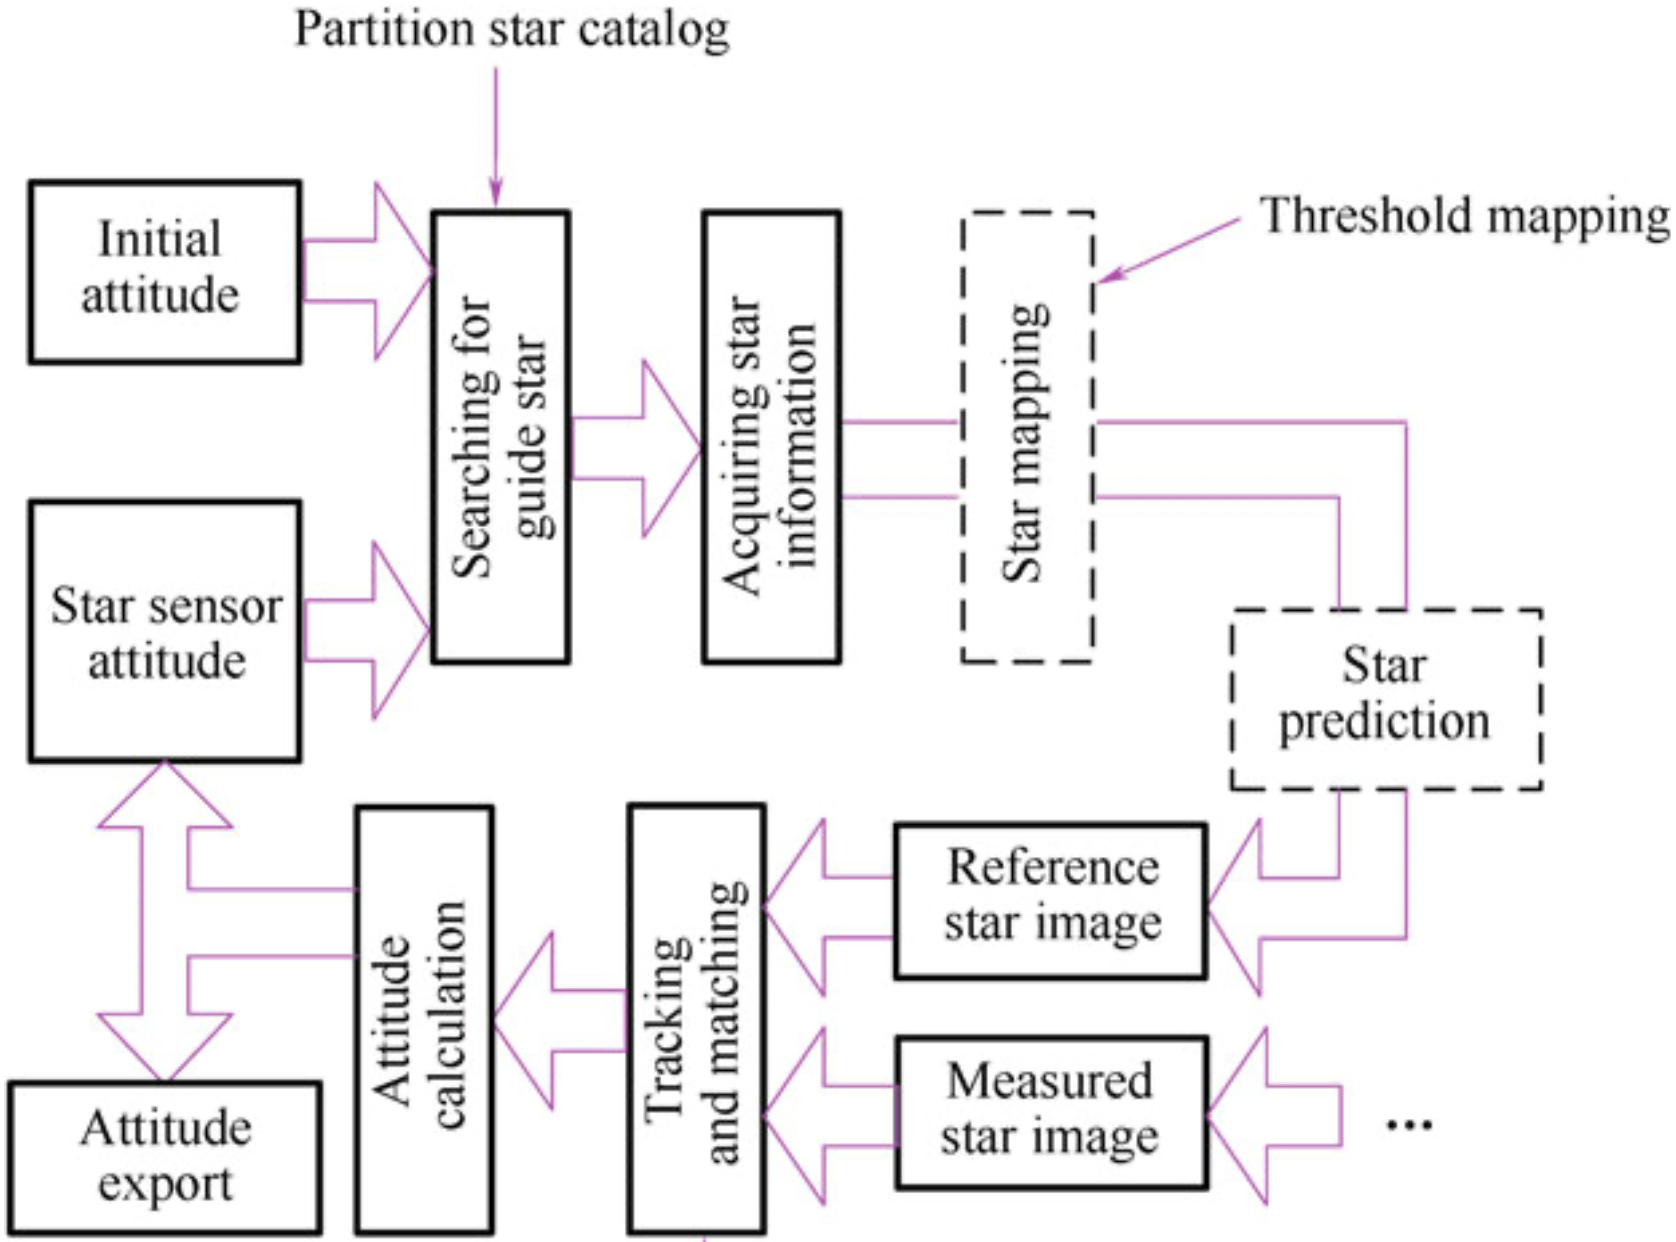
\includegraphics[scale=0.35]{Figures/GNC/zhang_tracking_flowchart.png}
        \caption{Star Tracking Algorithm}
        \label{fig:zhang_tracking_flowchart}
\end{Flowchart}

This algorithm also proposes three optimisation techniques to speed up the process of star tracking, where \textit{Sorting Before Matching} and \textit{Star Catalogue Partition} are the same as described before in algorithm \ref{rapidtrack}. The third technique, known as \textit{Threshold Mapping}, is explained below: 
\begin{itemize}
    \item \textbf{Threshold Mapping}\\ \label{threshold_mapping}
    In the process of Star Tracking, `Star Mapping' is the most time consuming process and executing it at every frame defeats the purpose of a tracking mode algorithm. \\
    In Threshold Mapping, a star number threshold, defined as $N_{\textit{TH}}$, is set. Star Mapping is not conducted unless the number of `Measured' stars tracked successfully is smaller than $N_{\textit{TH}}$. In this event, the measured image at the current frame, with the Star IDs identified, is used as the Reference Image for the next frame, after which Star Matching is carried out again as shown in Fig. \ref{fig:radius_zhang}. Hence, threshold mapping is adopted in order to reduce the frequency of star mapping. The process is shown in (\ref{fig:threshold_mapping}).
\end{itemize}
% PROBLEM : The figure shows \delta as the threshold whereas we have used Nth in the explanation. 
\begin{Flowchart}
        \centering
        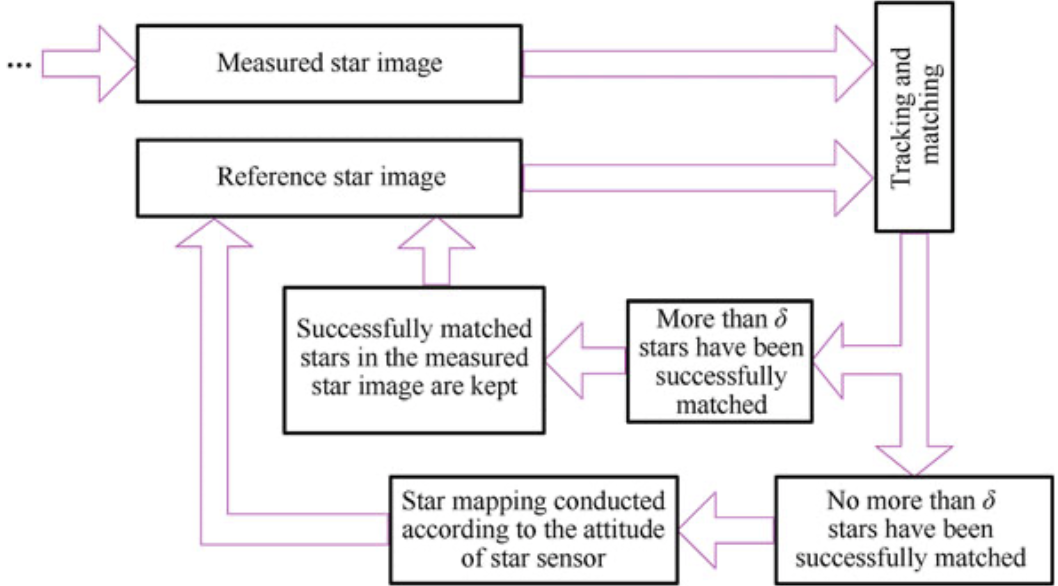
\includegraphics[scale=0.55]{Figures/GNC/threshold_mapping.png}
        \caption{Threshold Mapping}
        \label{fig:threshold_mapping}
\end{Flowchart}


\subsubsection{Fast Star Tracker Centroid Algorithm} \label{fast_algorithm}
This algorithm proposes a new star tracking algorithm, where the processes of Star Prediction and Star Matching are approached differently as compared to all algorithms discussed before. The algorithm does not require the use of a Gyroscope for obtaining the spacecraft angular velocity or the attitude information of any frame. Instead, the algorithm proposes an 'attitude independent' approach for estimating the angular velocity, i.e, the angular velocity can be estimated even without the attitude information of the current frame, and this estimated angular velocity is then used for centroid prediction. 
\begin{itemize}
    \item \textbf{Angular Velocity Estimation and Centroid Prediction}\\ \label{slew_prediction}
    The angular velocity estimate is obtained using only the centroid information of the previous \textbf{two} frames. 
    %The process is detailed below:
    % \begin{enumerate}
    %     \item Each star's unit vector can be calculated from its corresponding image plane coordinates by using the following formula:
    %     \begin{equation}
    %         \begin{bmatrix}
    %         x\\y\\z
    %         \end{bmatrix} = \frac{1}{\sqrt{u^2 + v^2 + f^2}} 
    %         \begin{bmatrix}
    %         u\\v\\f
    %         \end{bmatrix}
    %     \end{equation}
    %     where f is the lens focal length, and (u,v) are the image plane coordinates.
    %     \item Now, recalling Euler's Rotation Matrix (or Direction Cosine Matrix or DCM) from one reference frame to another: 
    %   \footnotesize{ \begin{equation}
    %         DCM = 
    %         \begin{bmatrix}
    %         cos(\psi)cos(\theta) & sin(\psi)cos(\theta) & -sin(\theta) \\
    %         -sin(\psi)cos(\phi)+ cos(\psi)sin(\theta)sin(\phi) & cos(\psi)cos(\phi)+sin(\theta)sin(\psi)sin(\phi) & cos(\theta)sin(\phi)\\
    %         sin(\phi)sin(\psi)+cos(\psi)sin(\theta)cos(\phi) & -cos(\psi)sin(\phi)+sin(\phi)sin(\theta)cos(\phi) & cos(\theta)cos(\phi)
    %         \end{bmatrix}
    %     \end{equation}
    %     }\\
    %     \normalsize 
    %     \begin{equation} \label{dcm_rotate}
    %         \begin{bmatrix}
    %         x\\y\\z
    %         \end{bmatrix} = DCM 
    %         \begin{bmatrix}
    %         x_{o}\\y_{o}\\z_{o}
    %         \end{bmatrix}
    %     \end{equation}
    %     where \textbf{$\phi$} is roll in radians about the x-axis, \textbf{$\theta$} is pitch in radians about the y-axis, and \textbf{$\psi$} is yaw in radians about the z-axis.  
        
    %     \item Assuming the small angle approximation, ($sin(\omega) = \omega$, $cos(\omega) = 1$ ; $\omega\psi = 0$; $\omega$ and $\psi$ $<<$ 1), \\
    %     Euler's equation can be reduced:
    %     \begin{equation}
    %         DCM \approx
    %         \begin{bmatrix}
    %         1 & \psi & -\theta \\ -\psi + \theta\phi & 1 + \theta\psi\phi & \phi \\
    %         \psi\phi+\theta & -\phi + \theta\psi & 1 
    %         \end{bmatrix} = 
    %         \begin{bmatrix}
    %         1 & \psi & -\theta \\ -\psi & 1 & \phi \\ \theta & -\phi & 1
    %         \end{bmatrix}
    %     \end{equation}\\
    %     Therefore, equation \ref{dcm_rotate} can be written as: 
    %     \begin{equation}
    %     \begin{bmatrix}
    %         x\\y\\z
    %     \end{bmatrix} = 
    %     \begin{bmatrix}
    %         1 & \psi & -\theta \\ -\psi & 1 & \phi \\ \theta & -\phi & 1
    %     \end{bmatrix}
    %     \begin{bmatrix}
    %         x_{o}\\y_{o}\\z_{o}
    %     \end{bmatrix}
    %     \end{equation}
        
    % \end{enumerate}
    Let the centroid of the $i_{th}$ star in the current frame and the previous frame be denoted by ($u_{i}(k)$, $v_{i}(k)$) and ($u_{i}(k-1)$, $v_{i}(k-1)$) respectively. Then the change in the u and v positions of the $i_{th}$ star is given by:
     \begin{equation} \label{slew_prediction_1}
        \begin{bmatrix}
         \Delta u_{i}(k) \\ \Delta v_{i}(k)
        \end{bmatrix} = 
        \begin{bmatrix}
        \frac{u_{i}(k-1)v_{i}(k-1)}{f} & -f \frac{u_{i}(k-1)^2}{f} & v_{i}(k-1) \\
        f + \frac{v_{i}(k-1)^2}{f} & -\frac{u_{i}(k-1)v_{i}(k-1)}{f} & -u_{i}(k-1)
        \end{bmatrix}
        \begin{bmatrix}
         \Phi(k) \\ \theta(k) \\ \Psi(k)
        \end{bmatrix}
     \end{equation}
     where \textbf{$\Phi$} is roll in radians about the x-axis, \textbf{$\theta$} is pitch in radians about the y-axis, \textbf{$\Psi$} is yaw in radians about the z-axis and f is the focal length.  \\ 
     Now equation \ref{slew_prediction_1} can be transformed to solve for the Roll, Pitch and Yaw given $\Delta u$ and $\Delta v$, and can be re-written as follows: 
     \footnotesize
     \begin{equation} \label{slew_prediction_2}
         \begin{bmatrix}
         \Phi \\ \theta \\ \Psi
        \end{bmatrix} = 
        \begin{pmatrix}
        \begin{bmatrix}
        \frac{u_{i}v_{i}}{f} & -f-\frac{u_{i}^2}{f} & v_{i} \\
        f+\frac{v_{i}^2}{f} & -\frac{u_{i}v_{i}}{f} & -u_{i}
        \end{bmatrix}^T
        \begin{bmatrix}
        \frac{u_{i}v_{i}}{f} & -f-\frac{u_{i}^2}{f} & v_{i} \\
        f+\frac{v_{i}^2}{f} & -\frac{u_{i}v_{i}}{f} & -u_{i}
        \end{bmatrix}
        \end{pmatrix}^{-1}
        \begin{bmatrix}
        \frac{u_{i}v_{i}}{f} & -f-\frac{u_{i}^2}{f} & v_{i} \\
        f+\frac{v_{i}^2}{f} & -\frac{u_{i}v_{i}}{f} & -u_{i}
        \end{bmatrix}^T
        \begin{bmatrix}
        \Delta u_{i} \\ \Delta v_{i}
        \end{bmatrix}
     \end{equation}
     
    \normalsize
     The centroid prediction process is carried out in the following steps:
     \begin{enumerate}
         \item The change in each stars' position from the previous image \emph{(k-1)} to the current image \emph{(k)} is calculated:
         \begin{equation}
             \Delta u_{i}(k) = u_{i}(k) - u_{i}(k-1); \Delta v_{i}(k) = v_{i}(k) - v_{i}(k-1)
         \end{equation}
         
         \item Equation \ref{slew_prediction_2} is solved to obtain the estimated roll, pitch and yaw of the optical detector. These values are the rotation angular rates from the previous frame to the current frame. Dividing these rates by the sensor's frame rate results in the estimated angular velocity. 
         \item A valid assumption here would be that the estimated rates between the previous frame \emph{(k-1)} and the current frame \emph{(k)} will be equal to the estimated rates between the current frame \emph{(k)} and the next frame \emph{(k+1)}. 
        \item Equation \ref{slew_prediction_1} can now be solved for $\Delta u(k+1)$ and $\Delta v(k+1)$, i.e, the change in the position of stars between the current frame \emph{(k)} and the next frame \emph{(k+1)}, using the estimated Roll, Pitch and Yaw obtained in the previous step. 
        \item Adding $\Delta u$ and $\Delta v$ to the position of stars at the current frame gives the \textbf{\emph{estimated}} positions of stars at the next frame (\emph{k+1}). 
     \end{enumerate}
     
     \item \textbf{Window Based Centroiding}\\ \label{subsec:window_matching}
     Window Based Centroiding is another approach for the \textbf{\emph{Star Matching}} process instead of the traditional Radius Based Matching as seen in Fig. \ref{fig:radius_zhang}. This approach can be described step-by-step as follows:
     \begin{enumerate}
         \item  After the process of Centroid Prediction, a \emph{Region-Of-Interest} (\emph{ROI}) / \emph{Window} of certain width is created around each predicted centroid, with the centroid as the center.
         \item The Region Growth algorithm (Refer \ref{subsec:fe_region_growth}) is now deployed in each of the windows to identify the 'true' centroid. 
         \item If only one centroid is identified in a window, the true centroid and the corresponding predicted centroid is matched.
         \item Steps 1 to 3 are repeated for all the remaining windows. 
     \end{enumerate}
     The window based centroiding is shown in Fig. \ref{fig:window_matching}
     \begin{figure}[!h]
        \centering
        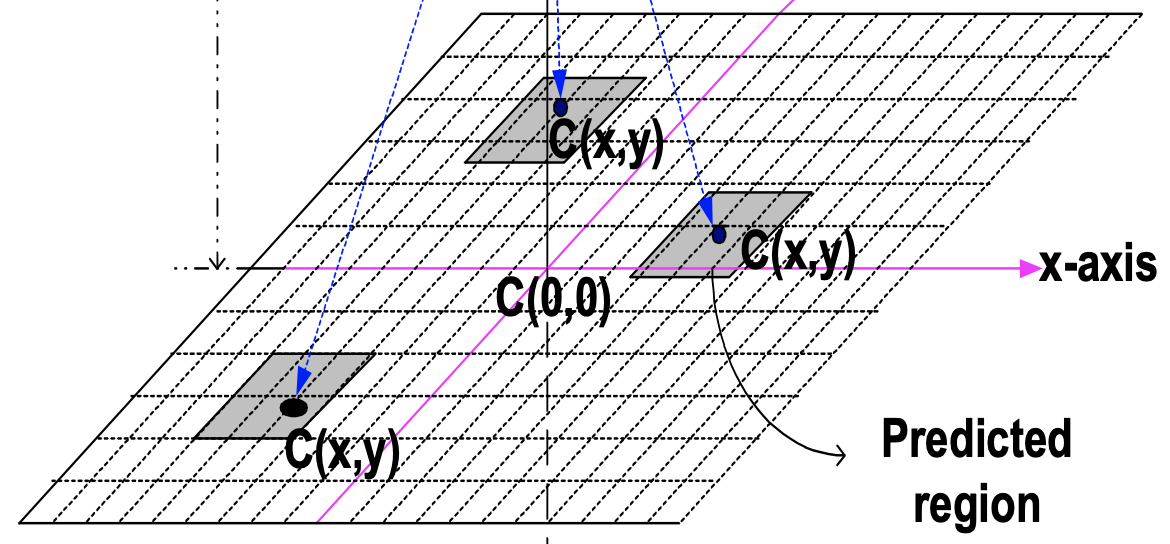
\includegraphics[scale=0.4]{Figures/GNC/window_matching.png}
        \caption{Window Based Centroiding}
        \label{fig:window_matching}
    \end{figure}
\end{itemize}
The algorithm at every frame checks whether the number of stars finally matched (either after LISA or tracking algorithm) are greater than or equal to \textbf{four}. At any given frame, if this condition is satisfied, the algorithm is executed, otherwise the particular frame is dropped and LISA is executed for the next frame. The algorithm can now be summarised as follows:
\begin{enumerate}
    \item The algorithm initialises to \textbf{State 1 (LIS Mode)}. State 1 runs the full frame centroiding on the input image and some stars are identified. The information of the identified centroids is stored as `Previous Centroids'. 
    \item If the number of previous centroids are greater than or equal to four, \textbf{State 10 (Transition mode)} is executed, which again runs full frame centroiding on the input image, resulting in the new centroids. The new centroids and the previous centroids are now passed into the `Assign IDs function'. 
    \item \textbf{`Assign IDs function'} \\
    This function identifies the new position of the previously identified stars to match the new centroids with the previous centroids. \\
    This is done by calculating the euclidean distance between each previous centroid and all new centroids, and the new centroid with the minimum distance is matched with the corresponding previous centroid. This process is repeated till all the previous centroids are matched.
    %% Write MaxDeltaUV using math-typesetting
    An upper threshold on the distance known as \emph{'MaxdeltaUV'} is kept to avoid false matching of new centroids entering or previous centroids exiting from the FOV. If less than two stars are matched between the two frames, or one star from the previous frame gets matched to more than one stars in the current frame, an error flag is generated and the algorithm return to State 1. 
    \item The centroids identified at the current frame are stored as `New centroids' and again checked if they are greater than or equal to four. If yes, the algorithm moves to \textbf{`State 2 (Tracking Mode)'}.
    \item State 2 passes the the centroids and IDs from the previous two images to the tracking code which predicts the location of the stars in the current image (Refer \ref{slew_prediction}). 
    \item The Window centroiding code uses the predicted centroid locations to find the new centroids in the current image (Refer \ref{subsec:window_matching}). If the matched stars are more than 4, the attitude is estimated, and `Previous centroids' and `New centroids' are updated for tracking stars in the next frames. If not, then state is reset to `State 1'. 
\end{enumerate}
The flowchart of the algorithm is as follows (\ref{fig:window_algorithm}):
\begin{Flowchart}
        \centering
        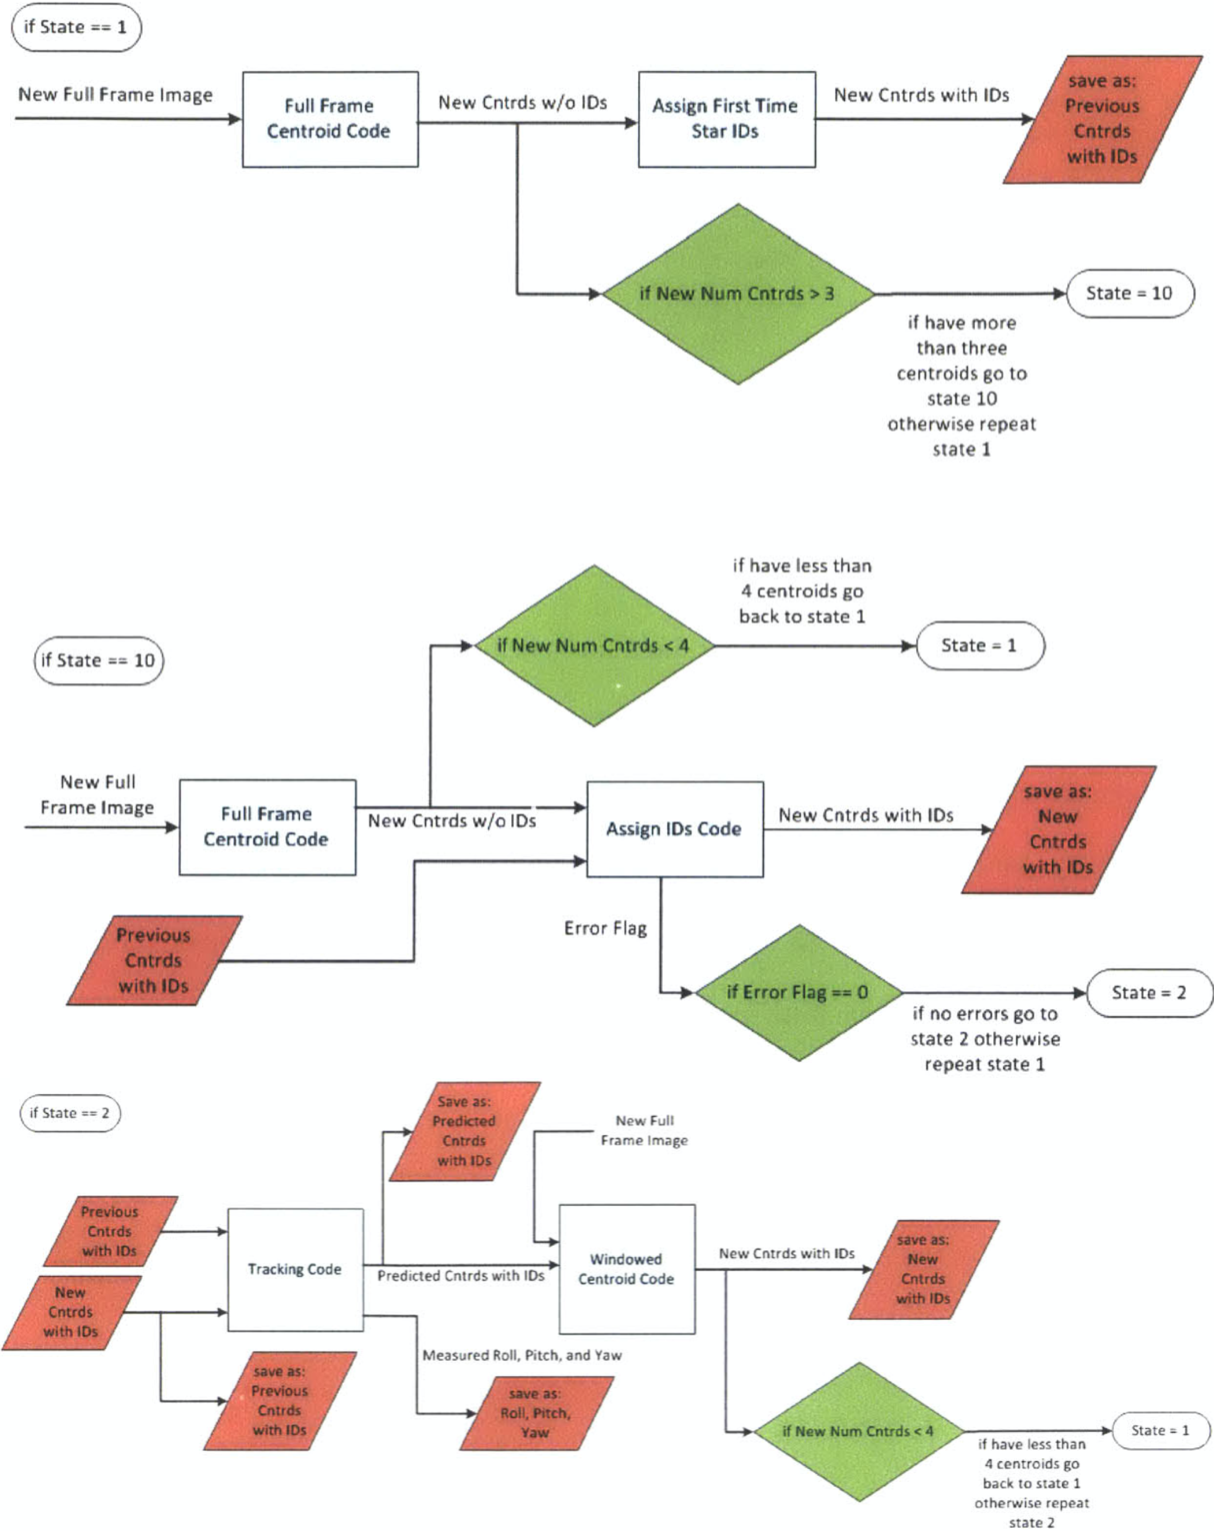
\includegraphics[scale=0.55]{Figures/GNC/window_algorithm.png}
        \caption{Fast Star Tracker Centroid Algorithm}
        \label{fig:window_algorithm}
\end{Flowchart}

\subsubsection{Current Tracking Mode Algorithm}
The Tracking Mode Algorithm finally decided by the team after going through all the above algorithms and more, takes some elements from each of the algorithms discussed previously. These elements include \emph{Centroid Prediction}, \emph{Radius based matching} and \emph{angular velocity estimation} (without Gyroscope). 
\begin{itemize}
    \item \textbf{Prediction v/s No Prediction}\\
    % Centroid prediction is the process of predicting the centroids of stars at the next frame, using the centroid information of previous frames or using an angular velocity estimate. The information of the predicted centroids, such as Star ID, RA and Dec value is already known. These predicted centroids form the \emph{'Reference Image'} and are then matched with the true centroids (which form the \emph{'Measured Image'}) obtained at the next frame, to perform Star Identification on the true centroids. 
    The process of matching stars between the Reference Image and the Measured Image is known as Star Matching. The process of constructing the Reference Image can be done in two different ways, with or without Centroid Prediction. Centroid Prediction/Star spot prediction is explained in section \ref{slew_prediction}. \\
    Using centroid prediction, the success rate of matching identification can be significantly improved in tracking and matching (Refer algorithm \ref{zhang}), as opposed to star matching without prediction (Refer algorithm \ref{rapidtrack}) \\
    This is mainly because of the ambiguity in the \emph{Matching Radius}, \textbf{r} in the latter algorithm, where a radius value too large or too small will result in a decrease in the number of matched and identified stars (Refer image \ref{fig:radius_zhang}). On the other hand, when centroid prediction is adopted, the radius value/window size is much smaller and equal to the centroiding error in the predicted centroids, as shown in Fig.\ref{fig:radius_based_sna}. \\
    It is important to note that the process of centroid prediction increases the amount of computation, and hence there is a trade off between speed and accuracy in this case. The team has finally decided to adopt centroid prediction in the final algorithm. 
    
    \item \textbf{Radius based v/s Window based Star Matching}\\
    Given the reference image (with prediction) and the measured image, `star matching' is deployed to match the centroids in the two images. Star matching again has two different approaches, namely the \emph{Radius based} (refer section \ref{rapidtrack}) and the \emph{Window based approach} (refer section \ref{subsec:window_matching}). \\
    The differences between the two approaches is as follows: 
    \begin{enumerate}
        %%% Include the flowchart you had made to explain the series and parallel nature of these operations
        \item In the radius based matching, both the Reference and the Measured Images are required to carry out Star Matching. Full Frame centroiding is adopted on the input image to form the Measured image. Centroid prediction is adopted to form the Reference Image. Both these processes run simultaneously and hence save computation time. Once the two images have been obtained, the process of star matching is carried out. 
        \item In the window based matching, first the reference image is formed by centroid prediction and then the window centroiding algorithm is deployed to look for the true centroids. In this case, the Measured image is not formed because of the absence of full frame centroiding, and hence the computation time decreases. But both the processes (prediction + window centroiding) run in series, so the computation time can increase.
        \item Since the radius based approach deploys full frame centroiding on the input image at the current frame, any new stars which may have entered into the FOV at the current frame will also be identified, thus making the algorithm more robust. This is not possible with the window based approach because centroiding occurs only around the predicted centroids and hence does not account for new stars entering into the FOV. 
    \end{enumerate}
    Taking into account the above points, the team has decided to design a Radius Based Star Matching algorithm in lieu of a Window Centroiding based Star Matching algorithm. 
    
    \item \textbf{Prediction with Gyroscope v/s Prediction without Gyroscope}\\
    The process of Centroid Prediction requires an estimate of the angular velocity and the centroids of the identified stars at the previous iteration. In algorithms \ref{sna} and \ref{zhang}, angular velocity is obtained using a Gyroscope, whereas in algorithm \ref{fast_algorithm}, the angular velocity is 'predicted' using the centroid information of previous two frames (refer section \ref{slew_prediction}). Since the team is not sure whether a Gyroscope will be compatible with the STADS system, the Centroid Prediction algorithm will be designed using the latter approach. 
\end{itemize} 
Before explaining the detailed steps of the algorithm, it should be noted that the Star Identification process has been completed for the current frame ($k^{th}$) and the previous frame ($k-1^{th}$). The task at hand is to identify stars at the next frame ($k+1^{th}$) using the Tracking Algorithm. The algorithm can now be described as follows: 
\begin{enumerate}
    \item The stars at the previous frame and the current frame are identified using LISA, and the corresponding centroids are stored as $N_{1}(k-1)$ and $N_{1}(k)$ respectively. If the number of common stars among $N_{1}(k-1)$ and $N_{1}(k)$ are greater than equal to 2, the execution of algorithm continues, otherwise LISA is performed in the next frame. 
    \item Angular Velocity is estimated using the set of centroids $N_{1}(k-1)$ and $N_{1}(k)$ after which the centroids at the next frame are predicted. (refer section \ref{slew_prediction} for more details). If no centroids were predicted, the algorithm switches back to LISA. The predicted centroids are stored as $N_{2}(k+1)$ and the \emph{Reference Image} is formed. 
    \item Alongside the process of centroid prediction, the algorithm runs full frame centroiding code at the next frame to form the \emph{Measured Image}. The centroids from the two images are now matched and identified using the `Radius based approach' for star matching (refer section \ref{rapidtrack}). The identified stars are stored as $N_{3}(k+1)$. 
    \item If $N_{3}(k+1)$ is greater than or equal to $N_{th}$, the identified stars are sent to the Estimation block for estimating the attitude and the Star ID process is finished. If $N_{3}(k+1)$ is less than $N_{th}$, the algorithm checks whether any new centroid was identified in the Measured Image which may have entered into the FOV. If yes, then the next step is executed, otherwise the tracking algorithm is terminated and LISA is deployed at the next frame. 
    \item To identify and match the new centroids at the next frame, the \textbf{\emph{Star Neighbourhood Table}} is used (refer section \ref{sna}). By referring to the SN Table, the unmatched neighbours of the identified stars in the next frame can be identified by comparing the inter-star angles between the stars in the Table and between the centroids in the Measured Image. Finally, the identified stars (after matching the new stars as well) are stored as $N_{4}(k+1)$. 
    \item Now, if $N_{4}(k+1)$ number of stars are greater than or equal to $N_{th}$, the star vectors are sent to the Estimation block and the Star ID process successfully ends. If $N_{4}(k+1)$ is still less than $N_{th}$, the Tracking algorithm is terminated and LISA is deployed at the next frame. 
\end{enumerate}
The algorithm is as follows  \ref{fig:tracking_flowchart}. 
\begin{Flowchart}
        %%% ADD new flowchart
        \centering
        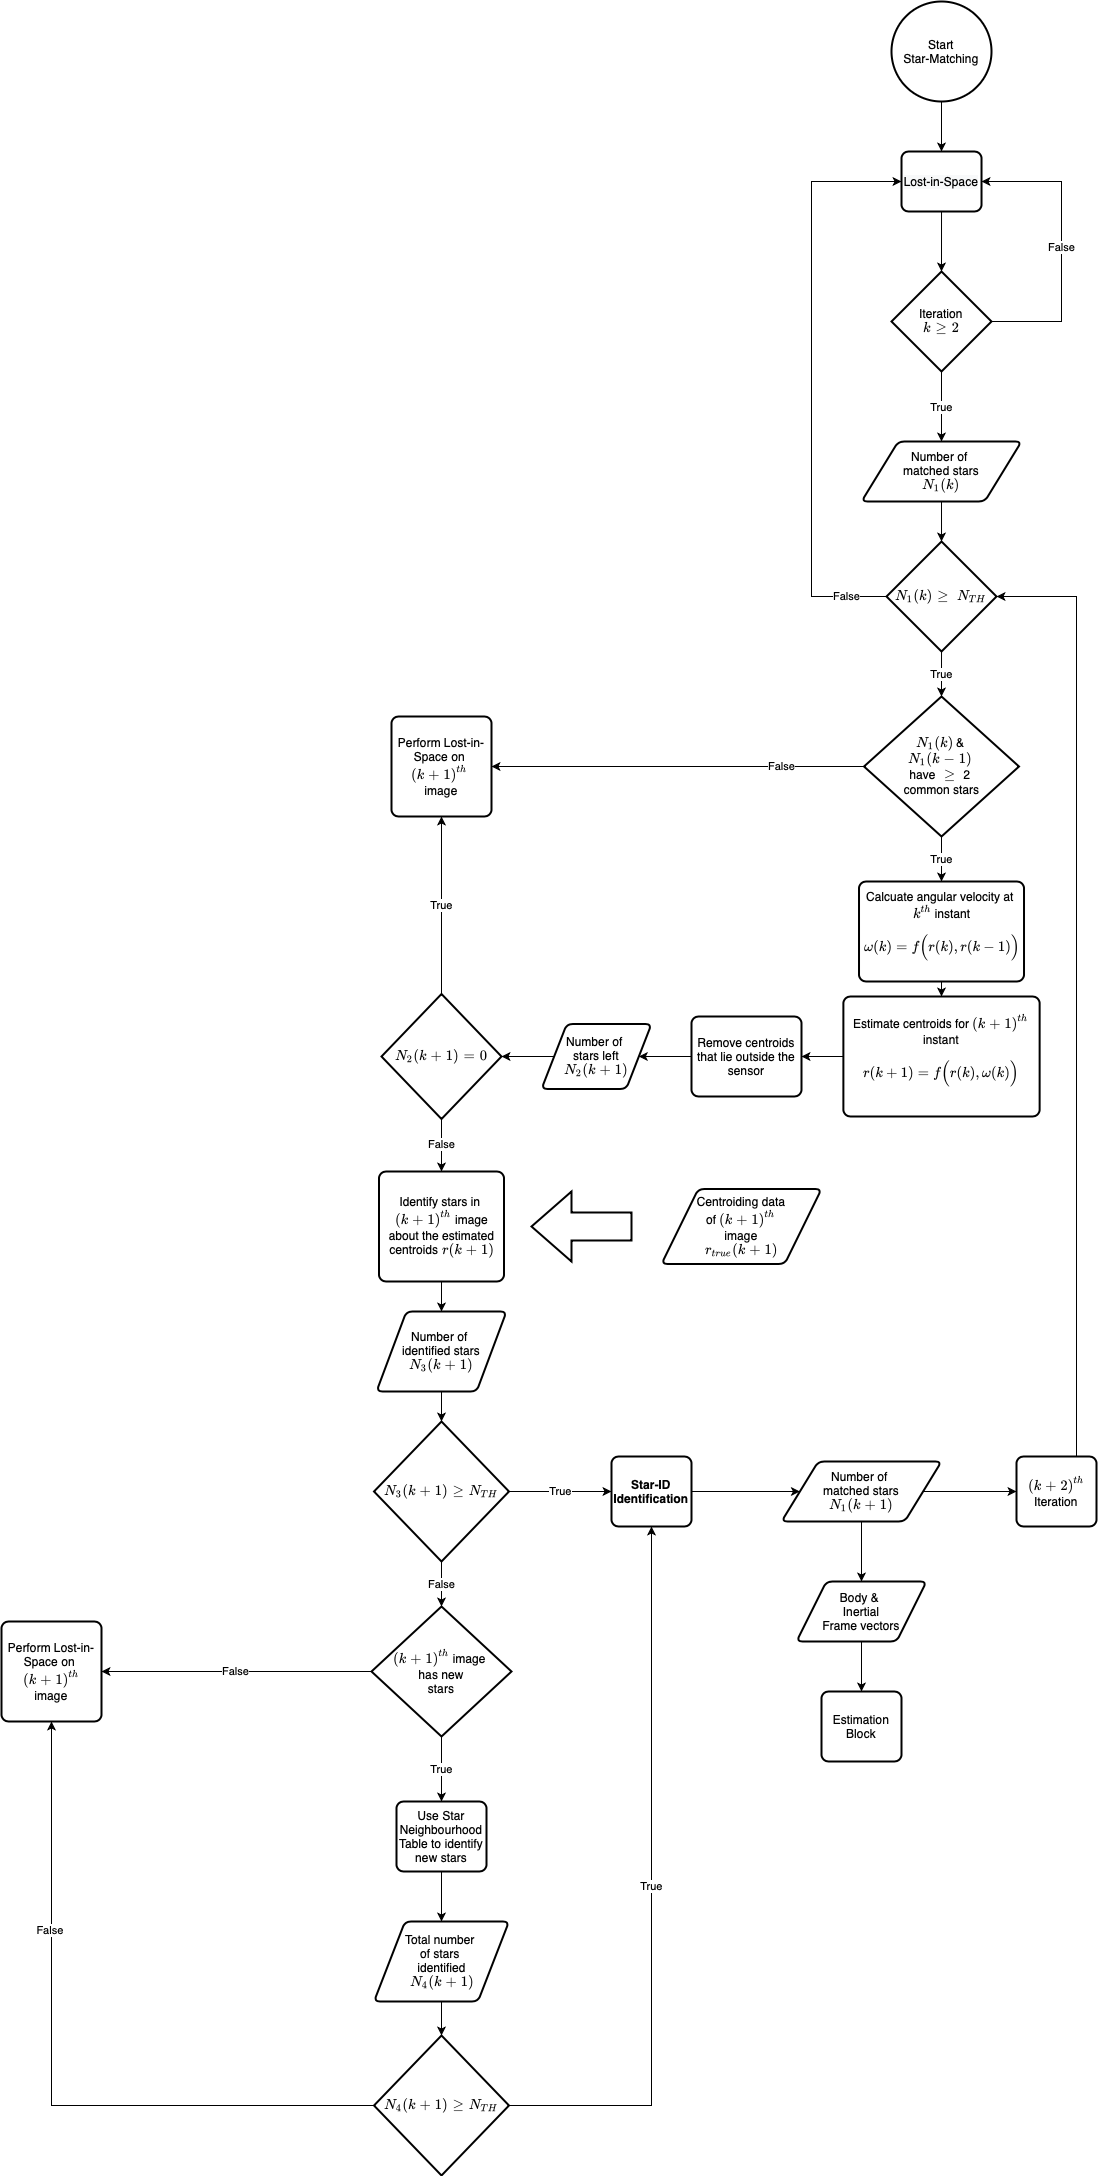
\includegraphics[scale=0.25]{Figures/GNC/tracking_flowchart.png}
        \caption{Current Tracking Algorithm}
        \label{fig:tracking_flowchart}
\end{Flowchart}
% Explain Nth. 
% Insert the Star Neighbourhood table
% Write the Future work. 
%----------------------------END----------------------------%
\end{document}